\subsection{Ejercicio 1}

\subsubsection{Segmentos de código, datos y de pantalla}
El sistema operativo utiliza dos segmentos de código de nivel 0 y 3, dos segmentos de datos de nivel 0 y 3 y un segmento que describe el área de la pantalla de video. Declaramos los cinco segmentos en la Tabla de Descriptores Globales (GDT), cada uno con su correspondiente descriptor. La GDT es un arreglo en memoria cuyas entradas ocupan 64 bits y tienen una estructura particular (ver figura 1). Para ingresar los datos con comodidad utilizamos un struct de C. La primer entrada está ubicada en la posición con índice 8. Todos los segmentos excepto el de video direccionan los primeros 500 MB de la memoria, es decir que se superponen.\newline
\begin{figure}[h]
\centering
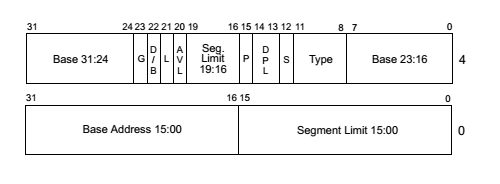
\includegraphics[scale=0.6] {descriptor_segmento}
\caption{Descriptor de segmento.}
\end{figure}
\begin{itemize}
\item Base, límite y granularidad: La base es 0x0, el límite es 0x1F3FF y la granularidad es 1. La granularidad activada hace que tratemos a la memoria como bloques de 4K, por lo tanto el límite con granularidad corresponde a la cantidad de bloques de 4K menos uno. Para direccionar los primeros MB, necesitamos la base en cero. El límite es 0x1F3FF porque en decimal es 127999, ya que necesitamos 128000 bloques de 4KB para llegar a 500 MB. Todo esto es para los segmentos de código y datos. Para descriptor de segmento de pantalla debemos especificar como base \verb|0xB8000| y para el límite necesitamos resolver (80 * 50 * 2) - 1, donde 80 es la cantidad de celdas, 1 celda == 2 bytes, en fila de pantalla y 50 es cantidad de celdas en columna. Es decir que el límite nos la cantidad de bytes que necesitamos para escribir en cualquier parte de la pantalla. Luego el valor del límite es \verb|0x1F3F|. La granularidad está cero ya que tiene menor tamaño (no necesita bloques de 4KB para direccionar toda su memoria).
\item Tipo: 0x0A en los segmentos de código (lectura, ejecución) y 0x02 en los segmentos de datos y de video (lectura, escritura).
\item Nivel de privilegios: 0x0 en los segmentos de datos y código que utiliza en kernel, así como en el segmento de video (que también es de uso exclusivo del kernel). Estos son los segmentos de nivel cero mencionados anteriormente. 0x03 en los segmentos de código y datos que utilizan las tareas, o sea el usuario, que corresponden a los segmentos de nivel tres mencionados anteriorente.
\item Sistema: 0x1 (que significa desactivado) pues no son segmentos de sistema sino de código y datos.
\item Presente: 0x1.
\end{itemize}

\subsubsection{Modo protegido y pila del kernel}
Realizamos los siguientes pasos:
\begin{itemize}
\item Habilitar A20 para poder acceder a direccioner superiores a $2^{20}$ bits.
\item Inicializar la GDT, cuyas entradas fueron ingresadas a partir de una dirección de memoria arbitraria, mediante la instrucción lgdt.
\item Activar el bit menos significativo de CR0.
\item Saltar a segmento:modoprotegido, donde segmento corresponde al índice del segmento de código de nivel 0 en la GDT corrido 3 ceros a la izquierda y modoprotegido corresponde a la dirección de memoria donde arranca el código que se ejecutará a continuación (ya en modo protegido).
\item Establecer los registros selectores de segmento datos (ds, es, gs y ss) en el índice del segmento de datos de nivel cero en la GDT corrido 3 bits a la izquierda.
\item Establecer el registro selector de segmento de video (fs) en el índice del segmento de video en la GDT corrido 3 bits a la izquierda.
\item Establecer la base de la pila en 0x27000.
\end{itemize}

\subsubsection{Limpieza e inicialización de la pantalla}
Para limpiar la pantalla hicimos una función en ensamblador que utiliza el segmento de video y otra en C que utiliza el segmento de datos. La función en ensamblador recorre byte por byte y la función en C recorre celda por celda (2 bytes) y llama a la función screen\_pintar en cada iteración. Ambas funciones dejan la pantalla en negro.\newline
Para inicializar la pantalla llamamos a la función screen\_inicializar que fue completada por nosotros, llamando a la función para limpiar la pantalla y luego a la función screen\_pintar\_rect para las distintas secciones.

